\documentclass[11pt]{article}
\usepackage{times}
\usepackage{fullpage}
\usepackage{url}
\usepackage{hyperref}
\usepackage{fancyhdr}
\usepackage{graphicx}
\usepackage{enumitem}
\usepackage{subcaption}
\usepackage{amsmath, amsfonts, amsthm, fouriernc}
\usepackage{IEEEtrantools}
\usepackage{parskip}
\usepackage{tikz}
\usetikzlibrary{positioning, calc, arrows.meta}
\usepackage{pgfplots}
\pgfplotsset{compat=1.16}

\pagestyle{fancy}
\addtolength{\headheight}{2em}
\addtolength{\headsep}{1.5em}
\lhead{\large{ME 2801}}

\usepackage{sectsty}
\sectionfont{\fontsize{12}{8}\selectfont}

\begin{document}

\begin{center}
  \Large{\bf{Assignment: Frequency Response and Bode Plots}}
\end{center}

% ---------------------------------------------------------------
\section*{Exercise 1: Ratio $\rightarrow$ Decibels}

The magnitude (AKA gain) of the transfer function is often expressed in decibels (dB) in the frequency response.  Express the following gain values in decibels:

\begin{enumerate}
\item $|G| = 1$
\item $|G| = 2$, \quad $|G| = 0.5$
\item $|G| = 10$, \quad $|G| = 0.1$
\item $|G| = 4.2$, \quad $|G| = 42$, \quad $|G| = 420$, \quad $|G| = 4200$
\end{enumerate}

% ---------------------------------------------------------------
\section*{Exercise 2: Decibels $\rightarrow$ Ratio: Closed-Loop Speed Response of the USV}

In the labs the USV autopilot controls forward speed with a feedback loop.  The input to the loop is the desired speed $R$ (m/s) and the output is the actual speed $Y$ (m/s), as shown in Figure~\ref{fig:speedloop}.  The plant is the surge model from Lab~1,
\[
  G(s) = \frac{5.1}{1.3\,s + 1},
\]
where the input is normalized throttle ($\pm 1$) and the output is forward speed (m/s).

\begin{figure}[h!]
  \centering
  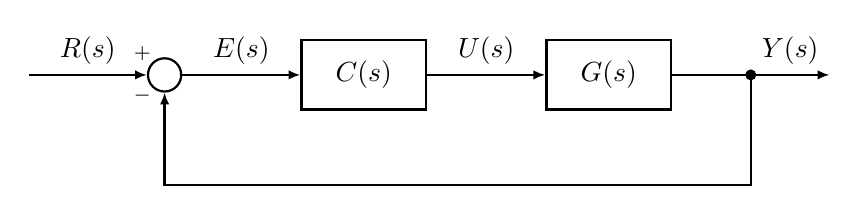
\begin{tikzpicture}[
    >={Latex[length=1.5mm, width=1.2mm]}, thick,
    block/.style = {draw, rectangle, minimum height=2.5em, minimum width=4.5em},
    sum/.style   = {draw, circle, inner sep=0pt, minimum size=1.2em},
  ]
    \node[coordinate]                    (rin)  {};
    \node[sum,   right=1.5cm of rin]     (sum)  {};
    \node[block, right=1.5cm of sum]     (C)    {$C(s)$};
    \node[block, right=1.5cm of C]       (G)    {$G(s)$};
    \node[coordinate, right=1.0cm of G]  (tap)  {};
    \node[coordinate, right=1.0cm of tap] (yout) {};
    \node[font=\scriptsize, inner sep=0pt, anchor=south east] at (sum.north west) {$+$};
    \node[font=\scriptsize, inner sep=0pt, anchor=north east] at (sum.south west) {$-$};
    \draw[->] (rin) -- node[above]{$R(s)$} (sum);
    \draw[->] (sum) -- node[above]{$E(s)$} (C);
    \draw[->] (C)   -- node[above]{$U(s)$} (G);
    \draw[->] (G)   -- node[above, pos=0.75]{$Y(s)$} (yout);
    \fill (tap) circle (2pt);
    \draw[->] (tap) -- ++(0,-1.4cm) -| (sum);
  \end{tikzpicture}
  \caption{USV speed loop: desired speed $R$ (m/s), throttle $U$ (normalized), actual speed $Y$ (m/s).}
  \label{fig:speedloop}
\end{figure}

The \emph{ideal} closed-loop response has a magnitude of one (0\,dB) at every frequency up to a cutoff frequency, so that the boat's speed follows the desired speed exactly, and then rolls off above the cutoff, so that the boat ignores commands (and noise) that change faster than it can or should respond.  Figure~\ref{fig:bodemag} shows the magnitude of the closed-loop frequency response, $G_{cl}(s) = Y(s)/R(s)$, for two controllers:
\begin{itemize}
\item Proportional only, $C(s) = K_P$, with $K_P = 0.2$ (the controller from the block diagrams assignment).
\item Proportional plus integral, $C(s) = K_P + K_I/s$, with $K_P = 0.2$ and $K_I = 0.45$.
\end{itemize}

\begin{figure}[h!]
  \centering
  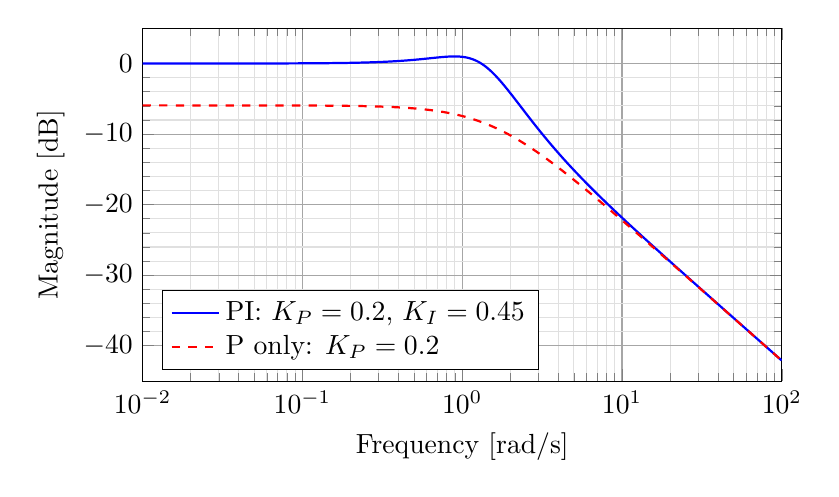
\begin{tikzpicture}
    \begin{semilogxaxis}[
      width=0.8\linewidth, height=0.5\linewidth,
      xmin=0.01, xmax=100, ymin=-45, ymax=5,
      ytick={-40,-30,...,0}, minor y tick num=4,
      grid=both,
      major grid style={black!35}, minor grid style={black!12},
      xlabel={Frequency [rad/s]}, ylabel={Magnitude [dB]},
      legend pos=south west, legend cell align=left,
      domain=0.01:100, samples=300,
    ]
      \addplot[blue, thick]
        {20*log10(5.1*sqrt((0.2*x)^2 + 0.45^2)
           / sqrt((5.1*0.45 - 1.3*x^2)^2 + (2.02*x)^2))};
      \addlegendentry{PI: $K_P = 0.2$, $K_I = 0.45$}
      \addplot[red, thick, dashed]
        {20*log10(1.02 / sqrt((1.3*x)^2 + 2.02^2))};
      \addlegendentry{P only: $K_P = 0.2$}
    \end{semilogxaxis}
  \end{tikzpicture}
  \caption{Magnitude of the closed-loop frequency response, desired speed to actual speed, for the USV speed loop.}
  \label{fig:bodemag}
\end{figure}

Suppose the desired speed varies sinusoidally about a steady cruising speed, with an amplitude of 0.5\,m/s.  Read the magnitude from Figure~\ref{fig:bodemag} to the nearest dB.

\begin{enumerate}
\item \textbf{PI control.}  Find the steady-state amplitude of the actual speed, with units, for each frequency of the desired speed:
  \begin{enumerate}
  \item 0.1\,rad/s (a period of about one minute)
  \item 1.0\,rad/s (a period of about 6\,s)
  \item 10\,rad/s (a period of about 0.6\,s)
  \end{enumerate}

\item \textbf{P-only control.}  Find the steady-state amplitude of the actual speed at 0.1\,rad/s.  How does the low-frequency magnitude of the P-only loop relate to the steady-state error you found for proportional control in the block diagrams assignment?

\item \textbf{Cutoff frequency.}  For the PI loop, estimate the frequency at which the magnitude drops to $-3$\,dB.  This is the cutoff frequency (bandwidth) of the speed loop.

%\item \textbf{Compare with the ideal.}  In two or three sentences, compare each curve with the ideal closed-loop response described above.  Where does each one match the ideal, and where does it fall short?
\end{enumerate}

% ---------------------------------------------------------------
\section*{Exercise 3: Bode Plots: Asymptotic Approximations}

Sketch the asymptotes of the Bode plot (magnitude and phase) for the following open-loop transfer functions.  Submit your hand sketch and identify the slope values for the asymptotes and the key values of the magnitude and phase plots.  You may use MATLAB to generate the Bode plots as a guide, but only submit your hand sketch.

Use the \href{https://bsb808.github.io/me2801/handouts/bode2_nolabel.png}{Bode graph paper} provided on the course website for sketching the frequency response.

For the magnitude plot, include labels for any non-zero slope values.

\begin{enumerate}
\item $L(s) = \dfrac{2000}{s + 200}$
%\item $L(s) = \dfrac{2000}{s\,(s + 200)}$ \quad (F\&P 6.3)
\item $G(s) = \dfrac{0.1}{s^2 + s + 4}$
%\item $G(s) = \dfrac{0.1\,(s + 10)}{s^2 + s + 4}$
\end{enumerate}

%Note: You can use the results from part 1 to build the Bode plot for part 2.  Similarly, you can use the result from part 3 to help generate part 4.

\end{document}
